% !TeX program = xelatex
% !TeX encoding = UTF-8
\documentclass[a4paper, 12pt, answers]{exam}

\usepackage[brazil]{babel}
\let\latinencoding\relax
\usepackage[T1]{fontenc}

\usepackage[no-math]{fontspec}
\usepackage{newpxtext, newpxmath}
\usepackage[a4paper, margin=2cm]{geometry}

\usepackage{siunitx}
\usepackage{fancyvrb}
\usepackage{graphicx}
\usepackage{caption}

\input{definition.tex}

\title{\titulo}
\author{\nomeAutorUm e \nomeAutorDois}
\date{\today}

\sisetup{
  binary-units = true
}

\renewcommand{\solutiontitle}{}

\fvset{
  gobble = 8,
  frame = single
}

\newcommand{\printtitle}{
  \begin{center}
    {\Large \scshape \titulo}\\[1em]
    {\nomeAutorUm, \raAutorUm}\\
    {\nomeAutorDois, \raAutorDois}\\[1em]
    Professor: Dr\@. \nomeProfessor, \centroProfessor\\
    {\itshape \campusFaculdade}
  \end{center}
}

\begin{document}
  \printtitle
  
  \begin{questions}
    \question
    Executar os diferentes servidores em uma máquina diferente da máquina cliente.
    
    \begin{parts}
      \part
      Usar o Visual VM para avaliar o comportamento dos programas em Java,
      incluindo o desempenho.
      
      \begin{solution}
        Pacote \verb|thread|: o servidor cria um \emph{thread} para cada nova
        conexão, liberando-o assim que o cliente desconecta. Desta maneira,
        permite-se com que múltiplos clientes possam se conectar a um mesmo
        servidor. A comunicação leva em média \SI{40}{\milli\second}. A criação
        e fechamento dos \emph{threads} está visível nas Figuras \ref{fig:thread-1}
        e \ref{fig:thread-2}, em que uma conexão nova é estabelecida criando-se 
        a \emph{thread} de número \verb|0|.
        
        \begin{Verbatim}[label={\$ java client.TCPClient}]
        Client> Este eh um teste
        Response: ESTE EH UM TESTE in 2 miliseconds.
        Client> Este eh um outro teste
        Response: ESTE EH UM OUTRO TESTE in 40 miliseconds.
        Client> quit
        \end{Verbatim}
        
        \begin{Verbatim}[label={\$ java thread.TCPServer}]
        Waiting for connection at port 9000.
        Connection established from 172.17.14.154, local port: 9000, 
        remote port: 51560.
        Waiting for connection at port 9000.
        From client 172.17.14.154:51560: Este eh um teste
        From client 172.17.14.154:51560: Este eh um outro teste
        Connection closed from 172.17.14.154:51560
        \end{Verbatim}
        
        \pagebreak
        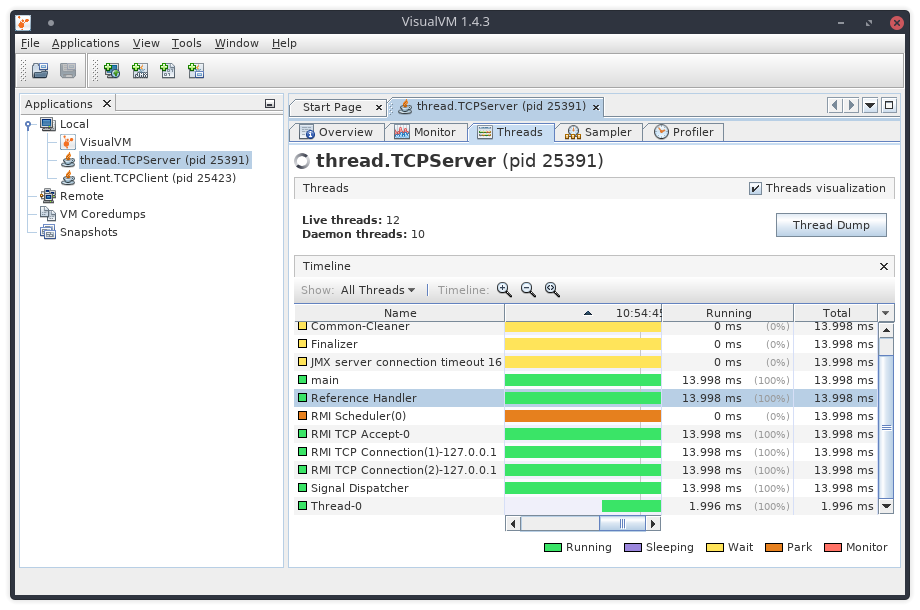
\includegraphics[width = \linewidth]{visualvm-01.png}
        \captionof{figure}{Início de uma \emph{thread} na aplicação Java \emph{threaded}.}
        \label{fig:thread-1}
        \vspace{1em}
        
        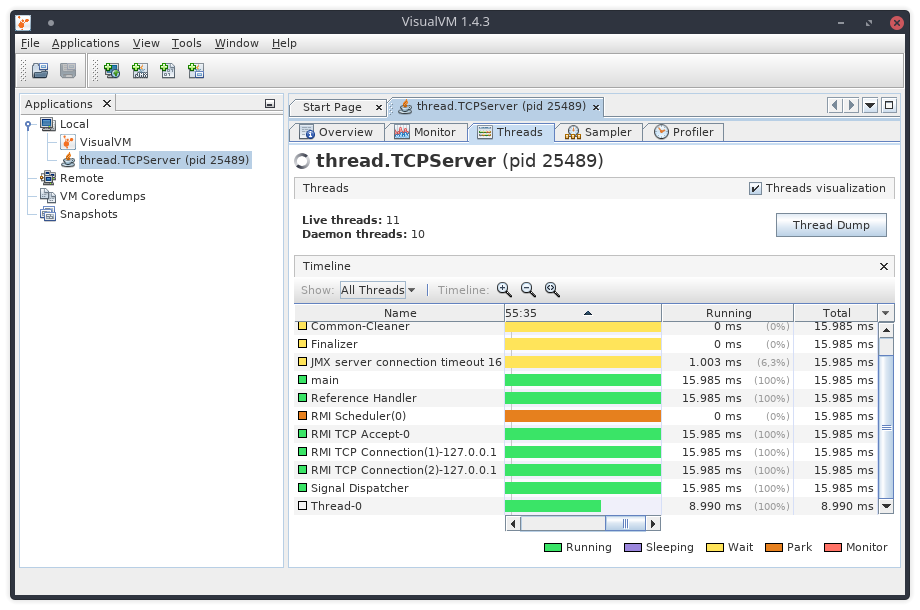
\includegraphics[width = \linewidth]{visualvm-02.png}
        \captionof{figure}{Fechamento de uma \emph{thread} ao término de uma conexão.}
        \label{fig:thread-2}
        \vspace{1em}
        
        Pacote \verb|nio|: cria-se um servidor não-bloqueante, através de um seletor 
        que fica monitorando os canais criados por cada nova conexão. Assim, toda vez
        que um cliente se conecta, registra-se ao seletor criando-se um canal a ser
        monitorado. O seletor tem como objetivo gerenciar múltiplas conexões (em 
        formas de canais) e múltiplos dados multiplexando esse processo.
        Logo após o início do programa, entra-se em um \emph{loop} infinito, 
        esperando por eventos, onde se aguarda novas conexões, além de ler e 
        escrever os dados no \emph{buffer}. Por utilizar uma máquina de estados
        finitos que controla o estado do \emph{buffer}, acaba-se gerenciando 
        da mesma maneira que o sistema operacional, por ser \emph{mono-threaded} 
        a eficiência torna-se maior, sem o \emph{overhead} que acompanha aplicações
        com diversas \emph{threads}. Entretanto, a estrutura do código e sua 
        compreensão e implementação se tornam consideravelmente mais complexas.
        A comunicação leva em média \SI{3}{\milli\second}.
        
        \vspace{.05em}
        \begin{Verbatim}[label={\$ java client.TCPClient}]
        Client> Este eh um teste
        Response: ESTE EH UM TESTE in 3 miliseconds.
        Client> Este eh um outro teste
        Response: ESTE EH UM OUTRO TESTE in 0 miliseconds.
        Client> quit
        \end{Verbatim}
        
        \vspace{.01em}
        \begin{Verbatim}[label={\$ java nio.TCPServer}]
        Waiting for connection at port 9000.
        Connection established from 172.17.14.154, local port: 9000, 
        remote port: 51616.
        From client /172.17.14.154:42150: Este eh um teste
        From client /172.17.14.154:42150: EFrom client 
        /172.17.14.154:51616: ste eh um outro  teste
        Connection closed from /172.17.14.154:42150
        \end{Verbatim}
        
        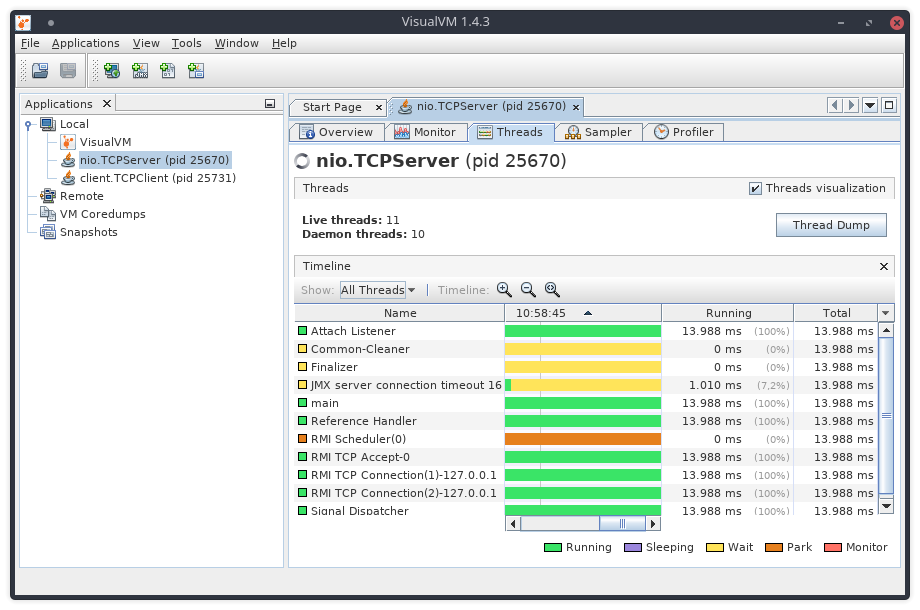
\includegraphics[width = \linewidth]{visualvm-03.png}
        \captionof{figure}{Pode-se visualizar que \emph{NIO} é \emph{mono-thread}.}
        \vspace{1em}
        
        Pasta \verb|fork|: cria-se uma fila de conexão, esperando por clientes.
        Assim, o \verb|listen| fica bloqueado. Esta implementação do servidor
        é \emph{mono-thread} e utiliza múltiplos processos, onde o processo 
        filho herda o \emph{socket} aberto do pai, processa-o e retorna,
        assim fechando o processo. A comunicação leva em média
        \SI{40}{\milli\second}. Inicialmente poderia ser suposto que por 
        se tratar de um programa escrito em C a performance teria de ser
        melhor que os desenvolvidos em Java, entretanto por cada conexão
        exigir a criação de um novo processo (algo extremamente caro em 
        recursos e tempo para o SO) a performance não apresenta melhora
        em relação a outras implementações.
        
        \begin{Verbatim}[label={\$ java client.TCPClient}]
        Client> Este eh um teste
        Response: ESTE EH UM TESTE in 1 miliseconds.
        Client> Este eh um outro teste
        Response: ESTE EH UM OUTRO TESTE in 40 miliseconds.
        Client> quit
        \end{Verbatim}
        
        \begin{Verbatim}[label={\$ ./fork/fork}]
        Waiting for connection at port 9000. 
        Waiting for connection at port 9000. 
        Connection established from 172.17.14.154, local port: 9000, 
        remote port: 51814.
        From client 172.17.14.154:51814: Este eh um teste
        From client 172.17.14.154:51814: Este eh outro teste
        From client 172.17.14.154:51814: quit
        Connection closed from 172.17.14.154:51814
        \end{Verbatim}
        
        % TODO: Precisa colocar as imagens da VisualVM e dos comandos abaixo.
        % \begin{Verbatim}[label={\$ ps aux | grep ./fork}]
        % \end{Verbatim}
        
        % \begin{Verbatim}[label={\$ pstree <PID>}]
        % \end{Verbatim}
      \end{solution}
      
      \part
      Fazer a captura dos pacotes usando Wireshark e discutir o protocolo de
      aplicação utilizado.
      
      \begin{solution}
       
        O protocolo de aplicação utilizado é o TCP (Transmission Control Protocol),
        um protocolo de comunicação em redes cujas propriedades garantem confiabilidade, 
        checagem de erros e manutenção da ordem dos pacotes que constituem uma mensagem.
        Uma das formas de proporcionar as propriedades citadas é a realização de um 
        \emph{handshake} de três vias, para estabelecer a conexão entre o servidor 
        e cliente, através do \verb|SYN| (pacote \emph{synchronize} enviado pelo 
        primeiro \emph{host}), \verb|SYN-ACK| (pacote \emph{synchronize-acknowledgment}
        enviado pelo segundo \emph{host}, reconhecendo que o pacote \verb|SYN| foi 
        recebido) e \verb|ACK| (pacote \emph{acknowledge} enviado novamente pelo
        primeiro \emph{host} reconhecendo que recebeu o pacote \verb|SYN-ACK|).
        Quando a comunicação é finalizada ocorre novamente um \emph{handshake} de 
        três vias para o fechamento da conexão o que garante novamente as 
        propriedades já citadas. O protocolo TCP também encapsula diversos
        outros protocolos de comunicação em redes, como FTP, HTTP, SMTP, POP3
        etc. Todos esse fatores fazem do TCP ser um protocolo de transmissão 
        confiável. É possível visualizar parcialmente o \emph{handshake} de três
        vias na Figura \ref{fig:wireshark-01}. Nesta captura de tela do Wireshark 
        é visível que a mensagem do pacote tem a primeira letra faltando: isso se 
        dá pois como parte do processo de \emph{handshake}, se utiliza o começo
        da mensagem a ser enviada neste processo. Também percebe-se a quebra da mensagem
        em diversos pacotes que são reconstituídos na ordem correta pelo protocolo TCP.
        
        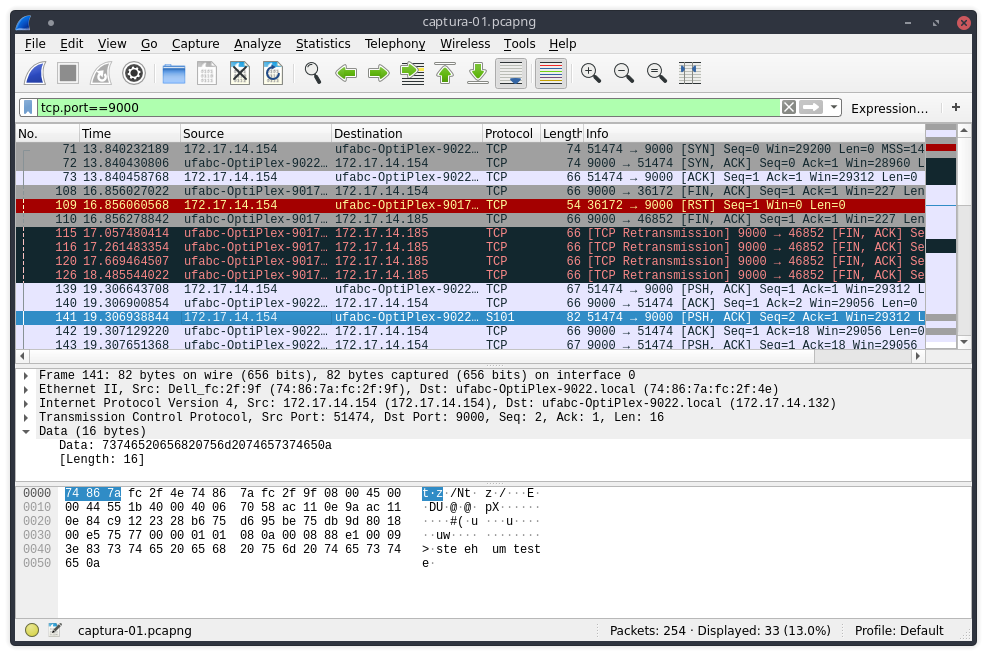
\includegraphics[width=\linewidth]{wireshark-01.png}
        \captionof{figure}{Comunicação entre cliente e servidor TCP com \emph{thread}.}
        \label{fig:wireshark-01}
        \vspace{1em}
        
        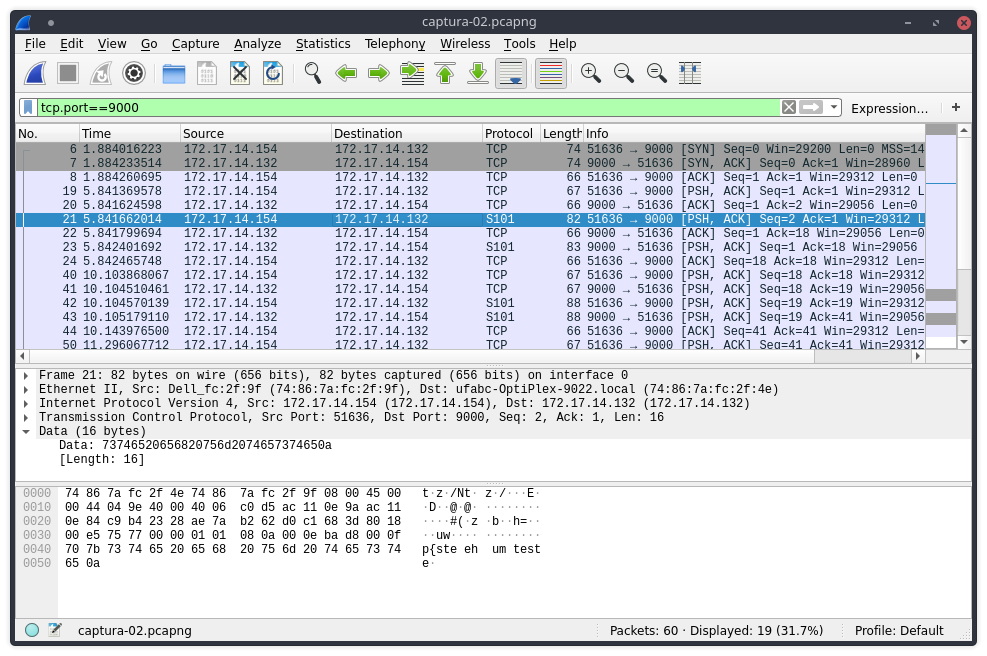
\includegraphics[width=\linewidth]{wireshark-02.png}
        \captionof{figure}{Comunicação entre cliente e servidor TCP não-bloqueante.}
        \vspace{1em}
        
        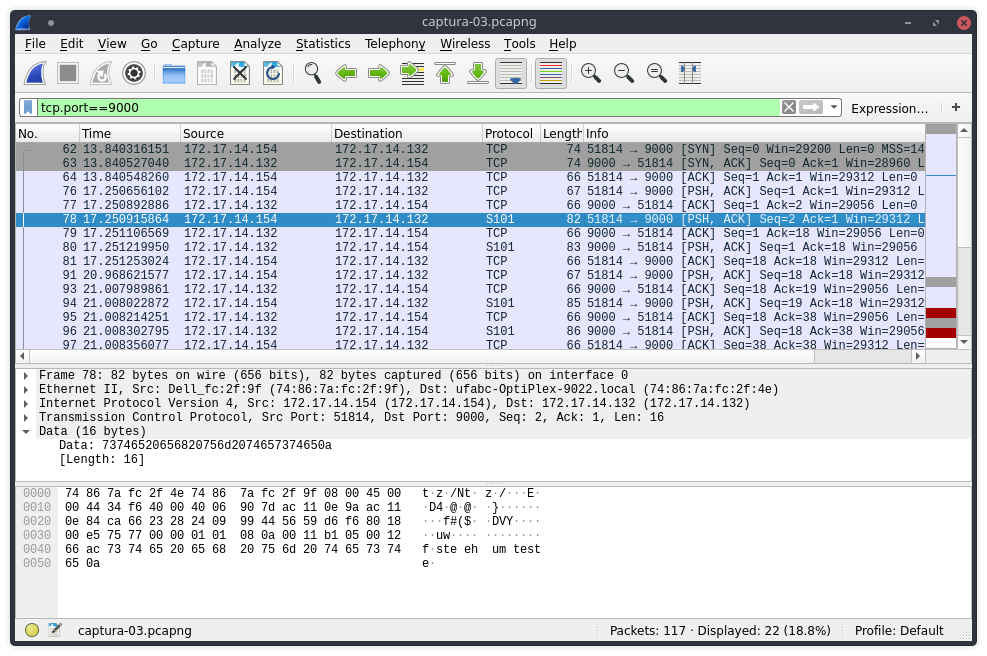
\includegraphics[width=\linewidth]{wireshark-03.png}
        \captionof{figure}{Comunicação entre cliente e servidor TCP com múltiplos processos.}
      \end{solution}
    \end{parts}
    
    \question
    Modificar o servidor Java \emph{multi-threaded} para usar pool de \emph{threads}.
    
    \begin{solution}
      Os códigos modificados se encontram no pacote \verb|pool| em anexo junto
      ao arquivo \verb|zip| deste relatório.
    \end{solution}
  \end{questions}
\end{document}